\section{Event Selections}
\label{sec:EventSelections}
%\todo[inline]{Give a brief overview of the three selections, even if they're unchanged from previous note, along with cut tables.}
%focus on changes with respect to the previous selection
%(Kate+Sophie

%\subsection{Preselections}

%The preselections employed are unchanged from the previous analysis and defined below.

This section describes the neutrino event selections in this analysis. These are the the electron (1e0p0$\pi$, 1eNp0$\pi$) and muon (1$\mu$0pX$\pi$) neutrino selections.  These selections are in large part unchanged from the run 1-3 analysis~\cite{PELEEnote}.  In particular the muon neutrino selection is identical.  The electron neutrino selection adds selection cuts related to the CRT on top of the previous selections to improve cosmic rejection, and further description is given in refCRTsection. Cut tables are included in Appendix A.  Validation of the selection over the full run 1-5 data set is described in section RefValidation.  

\subsection{CRT} %Work in progress - not ready for review yet
(Kate, work in progress)\\
The purpose of the CRT is to aid in reducing cosmic background in the analysis. CRT data will be employed for electron neutrino selections for run 3-run 5. The two main concepts the CRT relies on for cosmic reduction are veto cuts and distance cuts. CRT vetoing works by looking for coincidence between a beam flash and a CRT hit. That is, if a CRT hit occurs within 1 $\mu$s of a beam flash, the event is rejected. The other veto condition only considers CRT hits with PE \(>\) 100 photoelectrons. If either of these two conditions are met, the event is vetoed. These rely only on if the CRT is triggered in the beam window and how many photoelectrons are recorded, but the distance between CRT hits and the reconstructed neutrino vertex can also play a role. The CRT distance tagger works by tagging TPC tracks as cosmic-induced if the CRT hit and the track projection onto a CRT panel are within 5 cm of each other~\cite{PELEEnote}. The variables used for these CRT rejection cuts, as defined in ~\cite{PELEEnote}, are:\\
\\
\textbf{crtveto}: Boolean variable checking if the event passes the CRT veto.\\
\textbf{crthitpe}: How many photoelectrons (PEs) were recorded by the CRT system.\\
\textbf{\_closestNuCosmicDist}: 3D distance, measured in centimeters, between the reconstructed neutrino vertex and the closest CRT-tagged cosmic track.\\
\\
The CRT selection cuts that are applied to electron and muon neutrino selections in the analysis, defined by ~\cite{PELEEnote}, are as follows:

\begin{center}
    crtveto != 1  or crthitpe \(<\) 100 
\end{center}
\begin{center}
    \_closestNuCosmicDist \(>\) 5
\end{center}

Figures~\ref{fig:1eNp_preselection},~\ref{fig:1eNp_loosecuts},~\ref{fig:1e0p_preselection}, and~\ref{fig:1e0p_loosecuts} show the full effect of these CRT cuts when plotting events and reconstructed energy.

\begin{figure}[H] \centering
    \begin{subfigure}[t]{0.45\linewidth}
        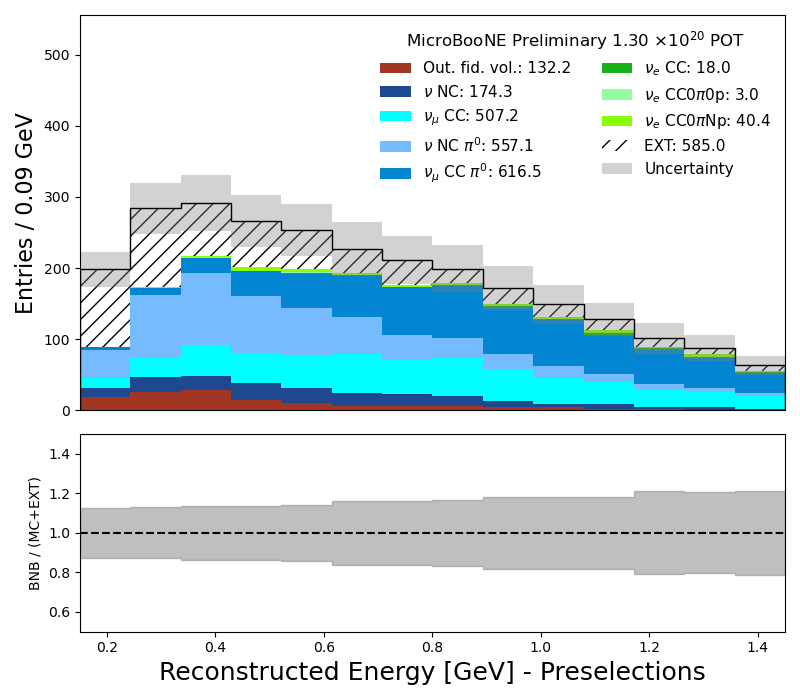
\includegraphics[width=\linewidth]{technote/EventSelections/FiguresCRT/run5_Np_presel.png}
        \caption{Reconstructed Neutrino Energy without CRT cuts}
    \end{subfigure}%
    \hspace{0.45cm}%
    \begin{subfigure}[t]{0.45\linewidth}
        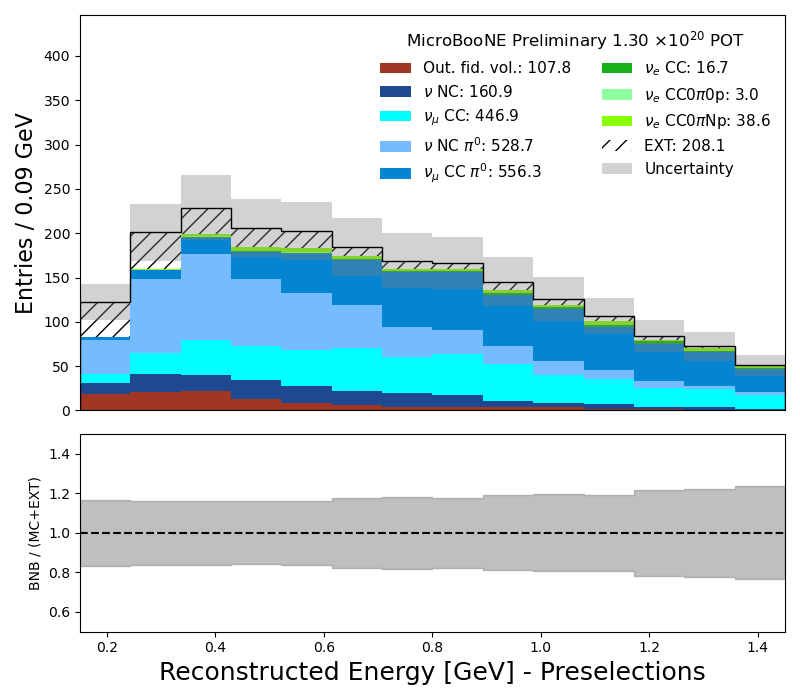
\includegraphics[width=\linewidth]{technote/EventSelections/FiguresCRT/run5_Np_presel_crt.png}%
        \caption{Reconstructed Neutrino Energy with CRT cuts}
    \end{subfigure}%
    \caption{Comparison of reconstructed neutrino energy for run 5 1eNp0$\pi$ preselection, with and without the application of CRT cuts to the event selection.}
    \label{fig:1eNp_preselection}
\end{figure}

\begin{figure}[H] \centering
    \begin{subfigure}[t]{0.45\linewidth}
        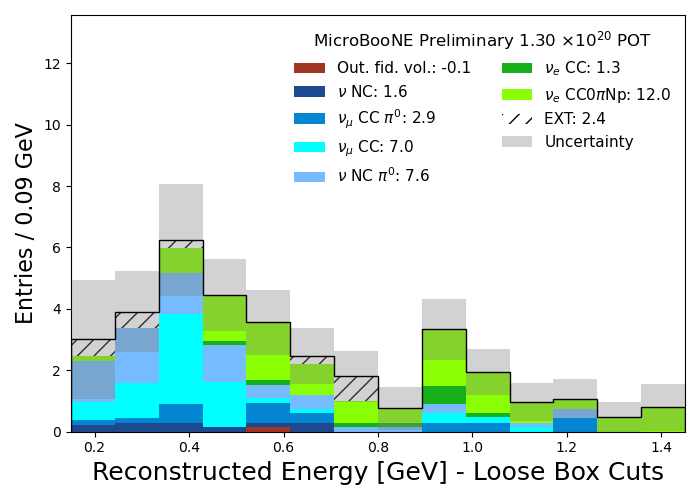
\includegraphics[width=\linewidth]{technote/EventSelections/FiguresCRT/run5_Np_loose.png}
        \caption{Reconstructed Neutrino Energy without CRT cuts}
    \end{subfigure}%
    \hspace{0.45cm}%
    \begin{subfigure}[t]{0.45\linewidth}
        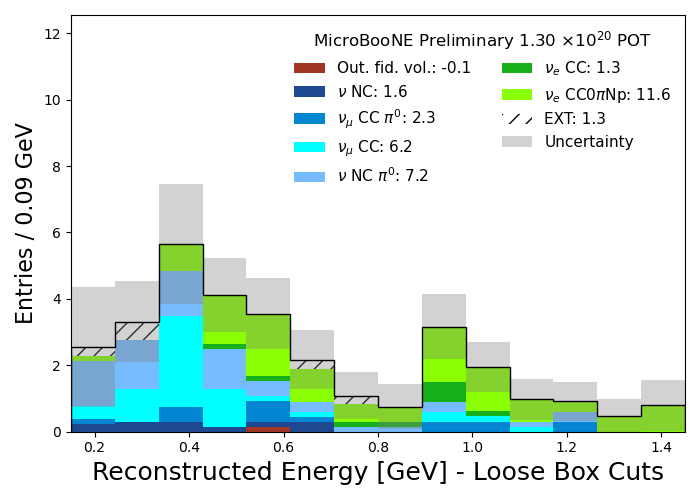
\includegraphics[width=\linewidth]{technote/EventSelections/FiguresCRT/run5_Np_loose_crt.png}%
        \caption{Reconstructed Neutrino Energy with CRT cuts}
    \end{subfigure}%
    \caption{Comparison of reconstructed neutrino energy for run 5 1eNp0$\pi$ loose box cuts, with and without the application of CRT cuts to the event selection.}
    \label{fig:1eNp_loosecuts}
\end{figure}

\begin{figure}[H] \centering
    \begin{subfigure}[t]{0.45\linewidth}
        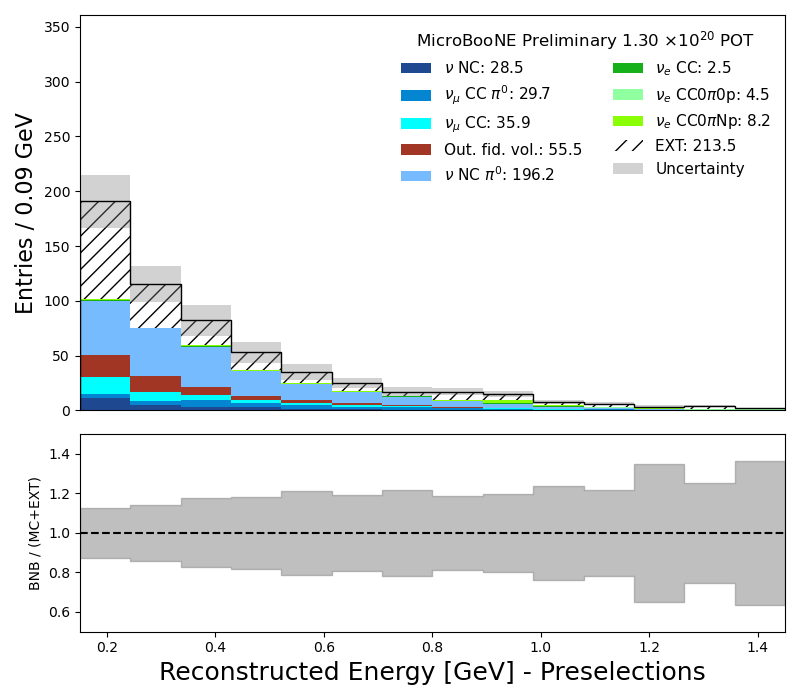
\includegraphics[width=\linewidth]{technote/EventSelections/FiguresCRT/run5_0p_presel.png}
        \caption{Reconstructed Neutrino Energy without CRT cuts}
    \end{subfigure}%
    \hspace{0.45cm}%
    \begin{subfigure}[t]{0.45\linewidth}
        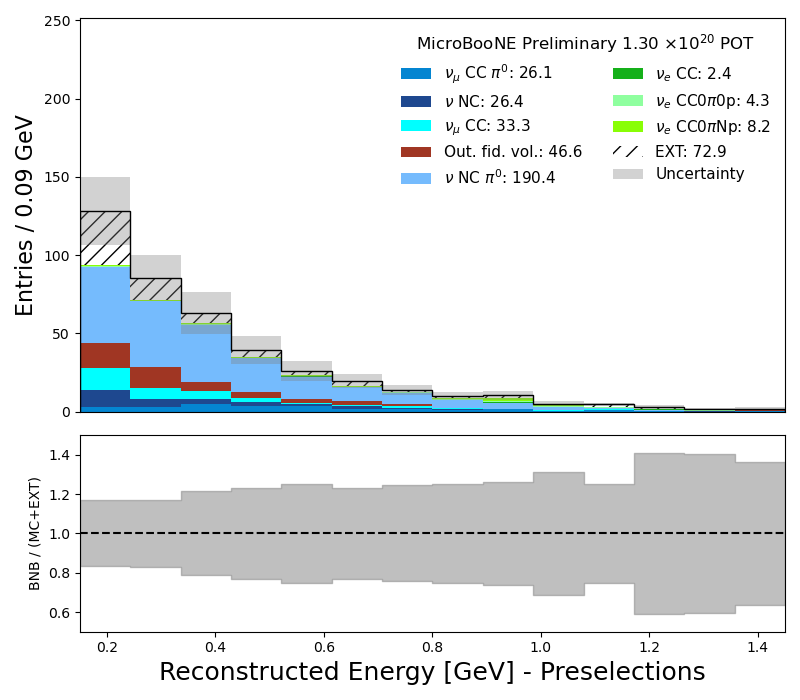
\includegraphics[width=\linewidth]{technote/EventSelections/FiguresCRT/run5_0p_presel_crt.png}%
        \caption{Reconstructed Neutrino Energy with CRT cuts}
    \end{subfigure}%
    \caption{Comparison of reconstructed neutrino energy for run 5 1e0p0$\pi$ preselection, with and without the application of CRT cuts to the event selection.}
    \label{fig:1e0p_preselection}
\end{figure}

\begin{figure}[H] \centering
    \begin{subfigure}[t]{0.45\linewidth}
        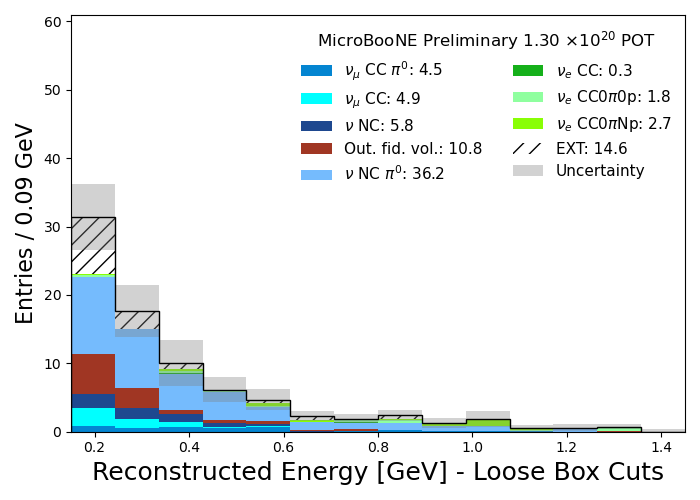
\includegraphics[width=\linewidth]{technote/EventSelections/FiguresCRT/run5_0p_loose.png}
        \caption{Reconstructed Neutrino Energy without CRT cuts}
    \end{subfigure}%
    \hspace{0.45cm}%
    \begin{subfigure}[t]{0.45\linewidth}
        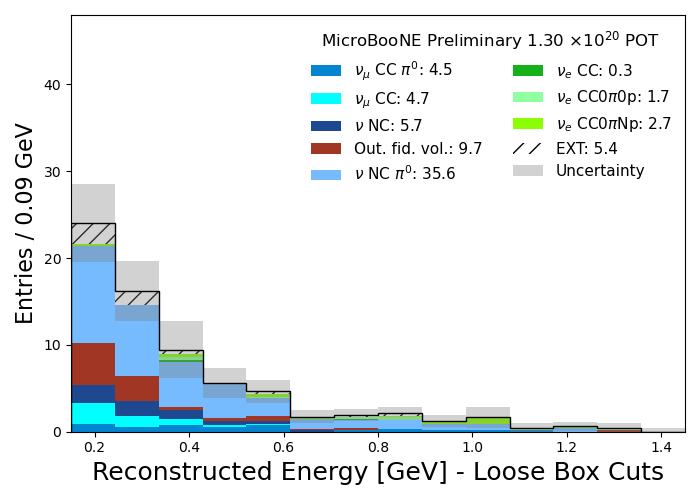
\includegraphics[width=\linewidth]{technote/EventSelections/FiguresCRT/run5_0p_loose_crt.png}%
        \caption{Reconstructed Neutrino Energy with CRT cuts}
    \end{subfigure}%
    \caption{Comparison of reconstructed neutrino energy for run 5 1e0p0$\pi$ loose box cuts, with and without the application of CRT cuts to the event selection.}
    \label{fig:1e0p_loosecuts}
\end{figure}

As the CRT is a new piece of hardware that has not been used over the full data set, it was necessary to check the time stability of EXT survival. This analysis was done by examining EXT vs. `run number' for run periods 3, 4b, 4c, 4d, and 5 with and without CRT cuts. We then take a ratio of EXT with CRT cuts and EXT without CRT cuts to acquire the rate at which cosmic events survive the CRT cuts. 

\begin{figure}[H]
 \centering
    \begin{subfigure}[t]{0.31\linewidth}
        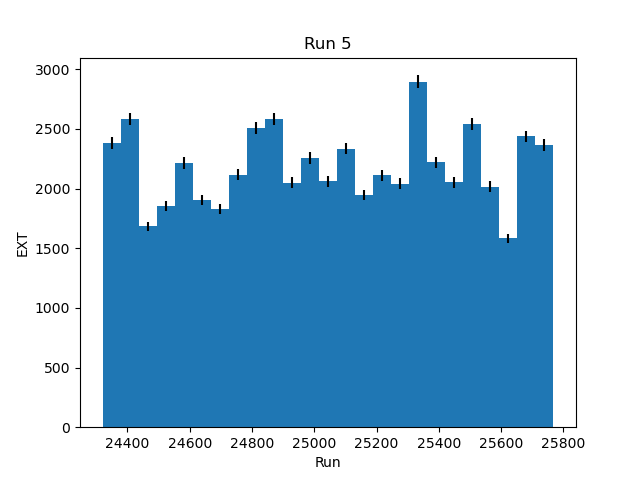
\includegraphics[width=\linewidth]{technote/EventSelections/FiguresCRT/run5_noCRT1.png}
        \caption{EXT vs. 'run' without CRT cuts}
    \end{subfigure}%
    \hspace{0.3cm}%
    \begin{subfigure}[t]{0.31\linewidth}
        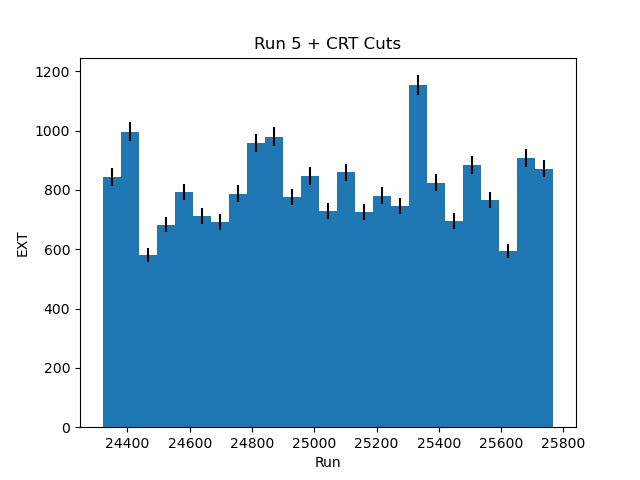
\includegraphics[width=\linewidth]{technote/EventSelections/FiguresCRT/run5_CRT1.png}%
        \caption{EXT vs. 'run' with CRT cuts}
    \end{subfigure}%
    \hspace{0.3cm}%
    \begin{subfigure}[t]{0.32\linewidth}
        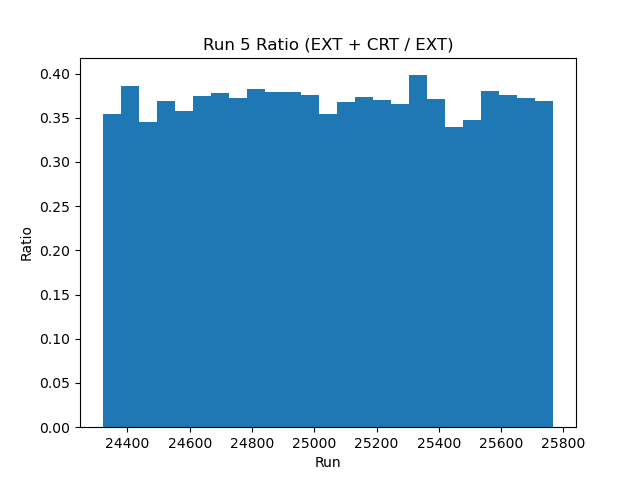
\includegraphics[width=\linewidth]{technote/EventSelections/FiguresCRT/run5fortalk.png}%
        \caption{Survival rate of EXT events}
    \end{subfigure}
    \caption{Analysis of EXT events vs. run number with overall event selection of `nslice==1', then with and without CRT cuts. The applied CRT cut here is `crtveto != 1'. Plot (c) shows the ratio of how many EXT events pass through the CRT cuts, or the survival rate. }
    \label{fig:EXT_survival_run5}
\end{figure}

Figure~\ref{fig:EXT_survival_run5} shows the ratio at which EXT events pass through the CRT cuts. To acquire the rejection ratio instead of the survival ratio, one can just take 1 - the survival rate. The above example shows the specific case of finding the survival rate using run 5 beam off data, with the selection of `nslice == 1', and the CRT cut `crtveto != 1'. 
This analysis was done for various CRT selection cuts as well as various neutrino selections. We examine each of the CRT variables individually, the veto variables separately, and then the entire CRT selection. For each of these CRT configurations, we examine the event selections of `nslice == 1', as well as electron neutrino preselection and muon neutrino preselection. The plots in Figures~\ref{fig:EXT_survival_run5} and~\ref{fig:EXT_survival_allruns} both use  the event selection `nslice == 1' and the CRT cut `crtveto != 1'. 
Figure~\ref{fig:EXT_survival_allruns} checks the stability of EXT survival by comparing the survival rate plots for run periods 3, 4b-d, and 5.

\begin{figure}[H]
 \centering
    \begin{subfigure}[t]{0.3\linewidth}
        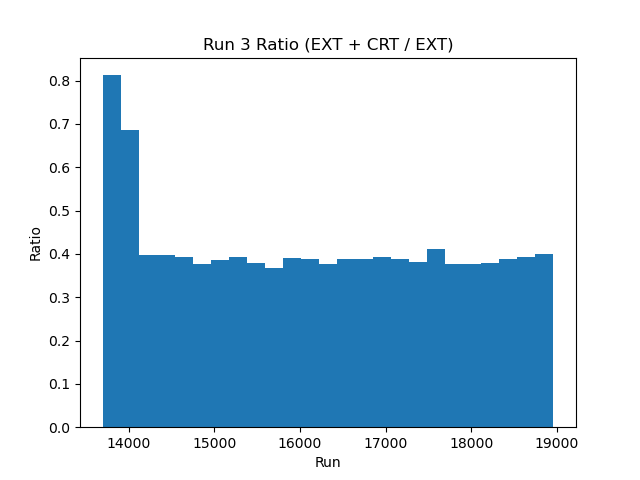
\includegraphics[width=\linewidth]{technote/EventSelections/FiguresCRT/run3_rationew.png}
        \caption{Survival rate of EXT events for run 3}
    \end{subfigure}%
    \hspace{0.3cm}%
    \begin{subfigure}[t]{0.3\linewidth}
        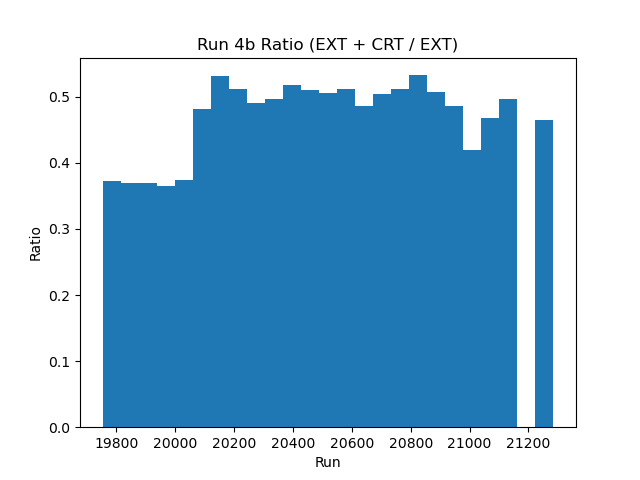
\includegraphics[width=\linewidth]{technote/EventSelections/FiguresCRT/run4b_ratio1.png}%
        \caption{Survival rate of EXT events for run 4b}
    \end{subfigure}%
    \hspace{0.3cm}%
    \begin{subfigure}[t]{0.3\linewidth}
        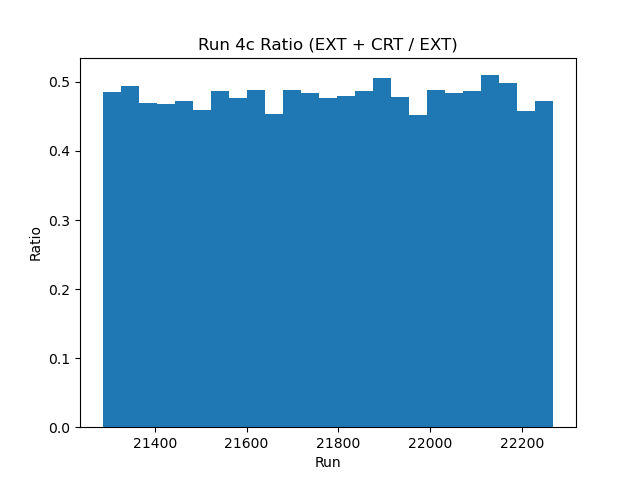
\includegraphics[width=\linewidth]{technote/EventSelections/FiguresCRT/run4cfortalk.png}%
        \caption{Survival rate of EXT events for run 4c}
    \end{subfigure}
    \hspace{0.3cm}%
    \begin{subfigure}[t]{0.3\linewidth}
        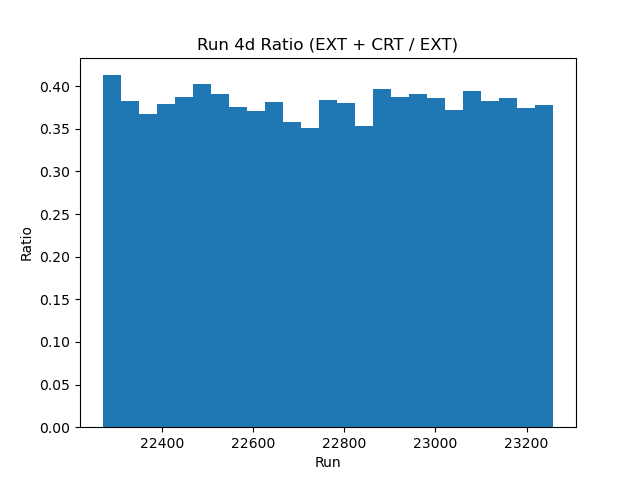
\includegraphics[width=\linewidth]{technote/EventSelections/FiguresCRT/run4dfortalk.png}%
        \caption{Survival rate of EXT events for run 4d}
    \end{subfigure}
    \hspace{0.3cm}%
    \begin{subfigure}[t]{0.3\linewidth}
        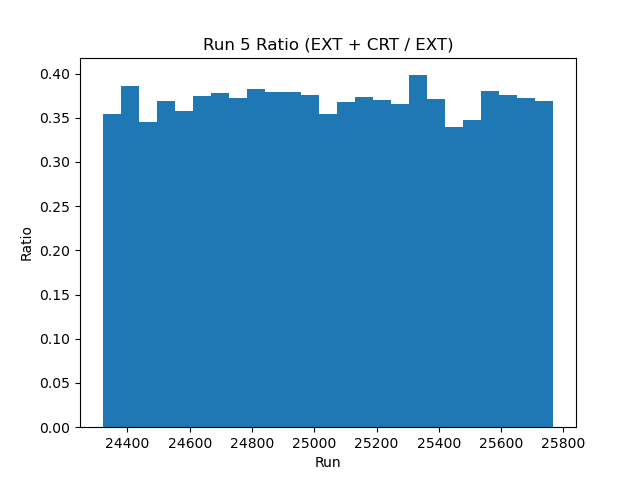
\includegraphics[width=\linewidth]{technote/EventSelections/FiguresCRT/run5fortalk.png}%
        \caption{Survival rate of EXT events for run 5}
    \end{subfigure}
    \caption{EXT event survival rates for runs 3, 4b-d, and 5. }
    \label{fig:EXT_survival_allruns}
\end{figure}

It is clear from Figure~\ref{fig:EXT_survival_allruns}, and this trend holds for the different CRT cut configurations and event selections, that the survival rate is not constant across these run periods. Regions of particular interest include the beginning of run 3, the step up in run 4b, and the drastic decrease in survival rate from run 4c to run 4d. This stability check revealed inconsistencies in the production of the beam off files in regards to the CRT variables. CRT-TPC merging was not performed correctly for some of the data sets and this led to this inconsistency ~\cite{Herb's presentation}. 

Once these fixes are made, we will once again check the time dependence and stability of EXT survival for various selections. Following these stability checks, the full analysis of 1eNp0$\pi$ and 1e0p0$\pi$ event selections can be done with the CRT included in selection cuts.

\subsection{Selection validation}
\label{sec:selvalid}
Describe validation of run 4 and 5 selection

\subsubsection{Comparison with Previous Framework}
\label{sec:compprevframework}

In order to check the consistency with the previous analysis, a range of checks were performed using various sample/event selection combinations. Three copies of each distribution were produced using three different versions of the code:
%
\begin{enumerate}
    \item The old analysis code, with the old data loading module (\verb|load_data_run123.py|) and the old plotting module (\verb|plotter.py|).
    \item The new data loading module (\verb|data_loading.py|), with the old plotting module.
    \item The new data loading and plotting modules.
\end{enumerate}
%
The outputs of these three module combinations are then compared, an example of this comparison is shown in Figures~\ref{fig:distvalidation_1e0p},~\ref{fig:distvalidation_1eNp}, and~\ref{fig:distvalidation_NuMu}\footnote{The minor discrepancy in the EXT in these plots can be explained by different approaches to the POT weighting when multiple runs are used. The new framework applies a POT scaling to the events from each individual run before combining them, whereas the old codebase would combine the runs together and then weight them.}.
%
\begin{figure}[H]
 \centering
    \begin{subfigure}[t]{0.32\linewidth}
        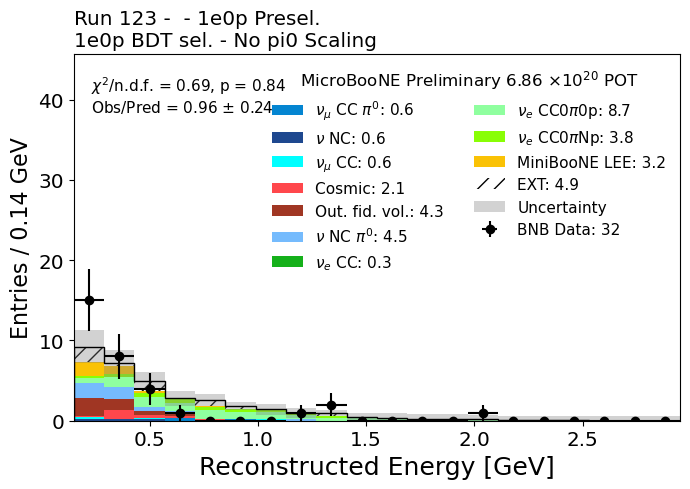
\includegraphics[width=\linewidth]{technote/EventSelections/Figures/Run123_1e0p_RecoEnergy_Old.png}
        \caption{Using the old data loading and plotting modules.}
    \end{subfigure}%
    \hspace{0.3cm}%
    \begin{subfigure}[t]{0.32\linewidth}
        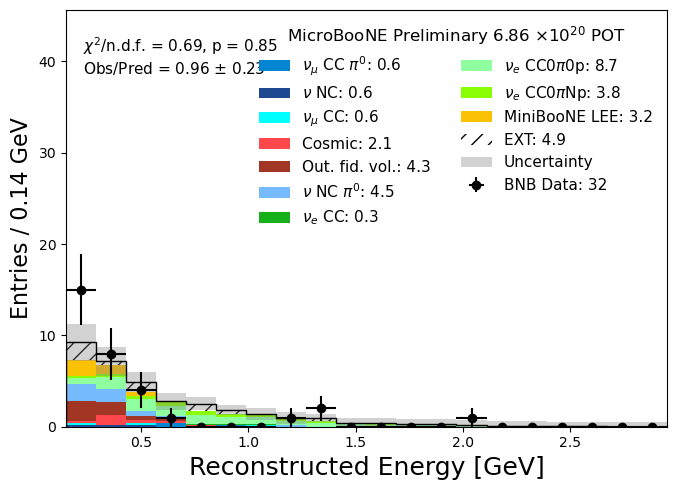
\includegraphics[width=\linewidth]{technote/EventSelections/Figures/Run123_1e0p_RecoEnergy_Chris.png}%
        \caption{Using the new data loading with the old plotting module.}
    \end{subfigure}%
    \hspace{0.3cm}%
    \begin{subfigure}[t]{0.31\linewidth}
        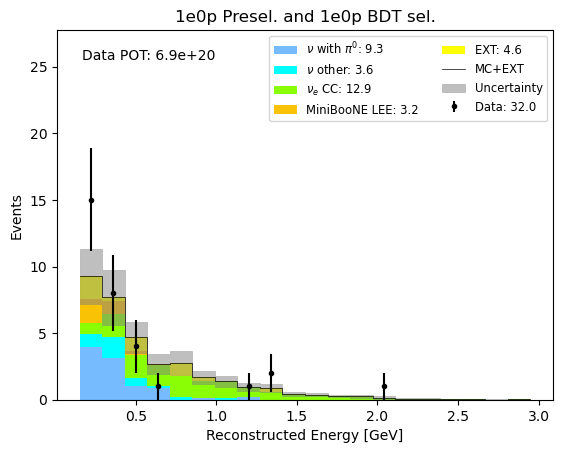
\includegraphics[width=\linewidth]{technote/EventSelections/Figures/Run123_1e0p_RecoEnergy_Alex.png}
        \caption{Using the new data loading and plotting modules.}
    \end{subfigure}% 
    \caption{Three copies of the reconstructed neutrino energy distribution produced with the three different module combinations for the purpose of software validation, using the full 1e0p event selection.}
    \label{fig:distvalidation_1e0p}
\end{figure}

\begin{figure}[H]
 \centering
    \begin{subfigure}[t]{0.32\linewidth}
        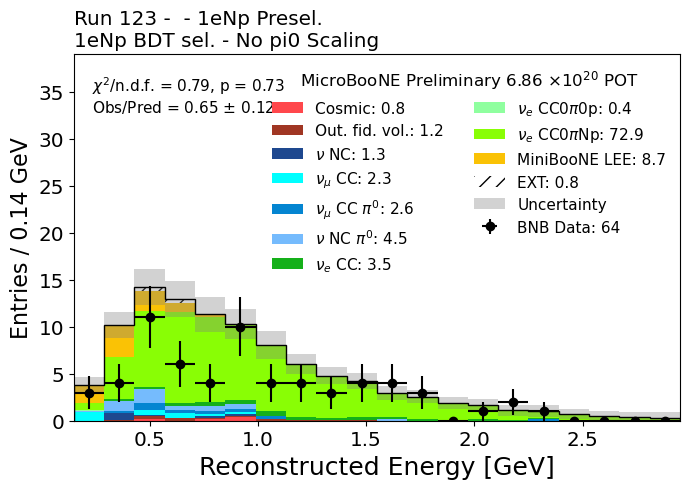
\includegraphics[width=\linewidth]{technote/EventSelections/Figures/Run123_1eNp_RecoEnergy_Old.png}
        \caption{Using the old data loading and plotting modules.}
    \end{subfigure}%
    \hspace{0.3cm}%
    \begin{subfigure}[t]{0.32\linewidth}
        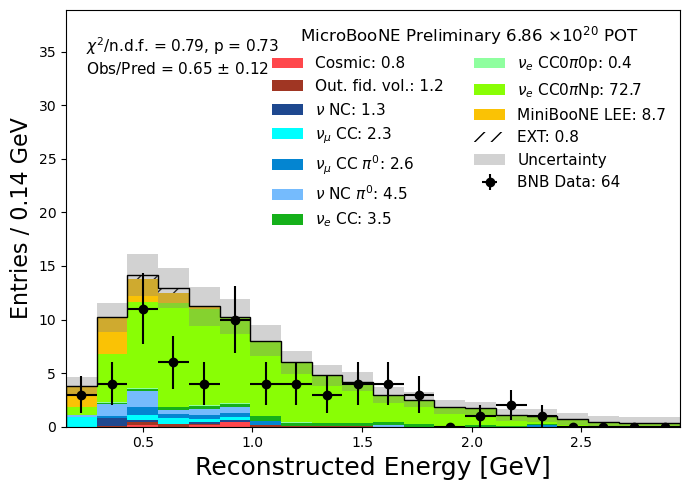
\includegraphics[width=\linewidth]{technote/EventSelections/Figures/Run123_1eNp_RecoEnergy_Chris.png}%
        \caption{Using the new data loading with the old plotting module.}
    \end{subfigure}%
    \hspace{0.3cm}%
    \begin{subfigure}[t]{0.31\linewidth}
        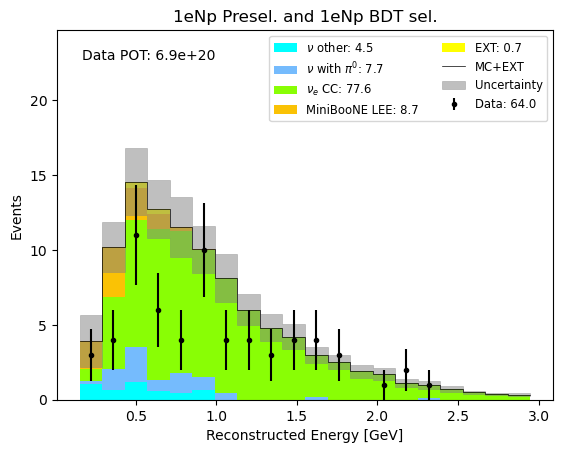
\includegraphics[width=\linewidth]{technote/EventSelections/Figures/Run123_1eNp_RecoEnergy_Alex.png}
        \caption{Using the new data loading and plotting modules.}
    \end{subfigure}% 
    \caption{Three copies of the reconstructed neutrino energy distribution produced with the three different module combinations for the purpose of software validation, using the full 1eNp event selection.}
    \label{fig:distvalidation_1eNp}
\end{figure}

\begin{figure}[H]
 \centering
    \begin{subfigure}[t]{0.32\linewidth}
        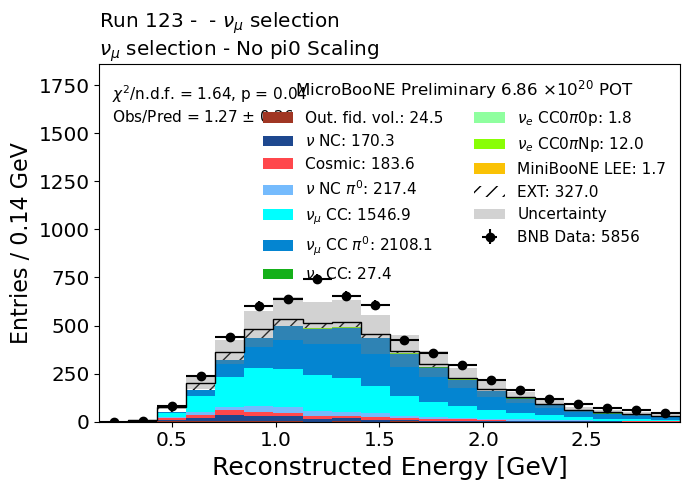
\includegraphics[width=\linewidth]{technote/EventSelections/Figures/Run123_NuMu_RecoEnergy_Old.png}
        \caption{Using the old data loading and plotting modules.}
    \end{subfigure}%
    \hspace{0.3cm}%
    \begin{subfigure}[t]{0.32\linewidth}
        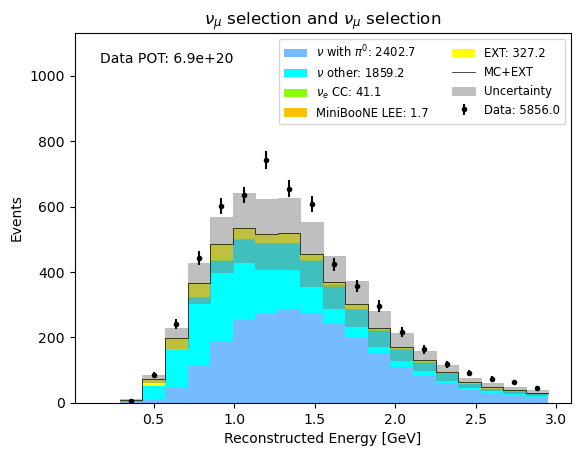
\includegraphics[width=\linewidth]{technote/EventSelections/Figures/Run123_NuMu_RecoEnergy_Alex.png}%
        \caption{Using the new data loading with the old plotting module.}
    \end{subfigure}%
    \hspace{0.3cm}%
    \begin{subfigure}[t]{0.31\linewidth}
        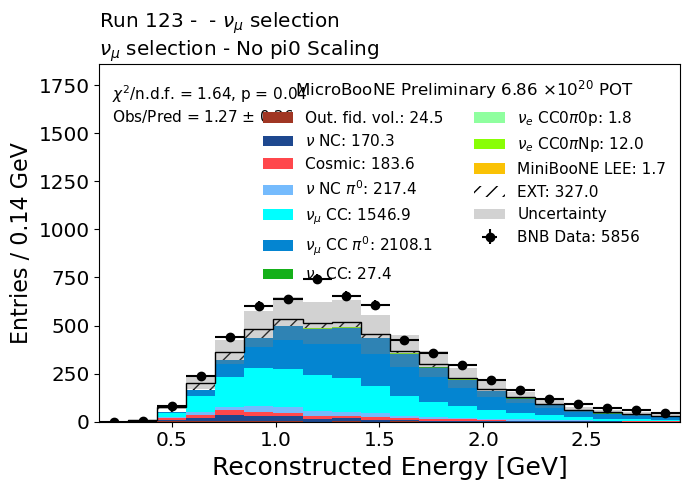
\includegraphics[width=\linewidth]{technote/EventSelections/Figures/Run123_NuMu_RecoEnergy_Old.png}
        \caption{Using the new data loading and plotting modules.}
    \end{subfigure}% 
    \caption{Three copies of the reconstructed neutrino energy distribution produced with the three different module combinations for the purpose of software validation, using the full $\nu_{\mu}$ event selection.}
    \label{fig:distvalidation_NuMu}
\end{figure}

Show consistency across runs
Compare variables across runs, data/MC plots 
For example, runs 123 compared to run 4 and 5 separately

Check things like consistency of calorimetry, rate of cosmics, inputs into the BDT
Fan's plots for run 4 and 5 validation (Fan)